\subsection{Chord}
\label{chap:evaluation_chord}

\subsubsection{Aufbau und Struktur}
Chord \cite{Stoica2003} legt die $l$ bit wertigen Schlüssel (meist Zahlen im Bereich $[0,2^l-1]$) auf einem eindimensionalen Ring modulo $2^l$ im Uhrzeigersinn an. Jedem Knoten und jedem Datum ist ein eindeutiger Schlüssel zugewiesen, diese werden \emph{ID} und \emph{key} genannt. Ein Datensatz $X$ ist dem Knoten zugewiesen, dessen ID größer gleich dem key ist. Dieser Knoten wird Nachfolger von X, \emph{SUCC(X)}, genannt. Analog dazu gibt es auch einen Vorgänger von X, \emph{PRED(X)}.

\begin{figure}[htbp]
\centering
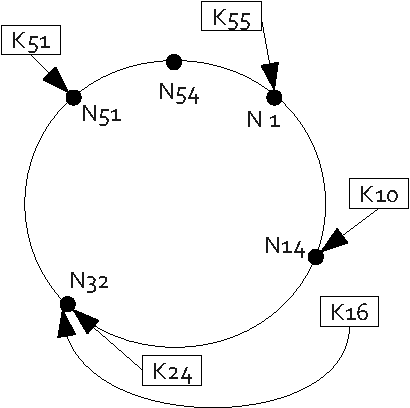
\includegraphics{grafics/chord_key_space.pdf}
\caption{Schlüsselraum für Chord mit sechs Knoten ($Nx$) und fünf Daten ($Kx$)}
\label{fig:chord_key_space}
\end{figure}

Damit ist ein Knoten für alle Daten zuständig, die -- bildlich gesehen -- im Ring gegen den Uhrzeigersinn vor ihm liegen. In \Fref{fig:chord_key_space} ist dies mit $l=6$ für sechs Knoten und fünf Datenpunkten gezeigt. Knoten 14 (N14) ist für den Datensatz mit Schlüssel 10 (K10) zuständig. Knoten 32 ist für K16 und K24 verantwortlich. K51 ist bei N51 zu finden. Aufgrund der Ringstruktur ist N1 für K55 zuständig. Die gestrichelten Pfeile stellen die Einträge der sogenannten Fingertabelle für Knoten $N1$ dar. 

\subsubsection{Routing}
Bei Chord besitzt jeder Knoten eine Verbindung zu seinem direkten Vorgänger und seinem direkten Nachfolger. Eine Nachricht wird von jedem Knoten so lange an seinen Nachfolger geschickt, bis sie zum zuständigen Knoten gelangt. Bei einer \texttt{lookup(x)}-Nachricht\footnote{Suche für key x Knoten N, so dass gilt: $N = SUCC(x)$.} prüft jeder involvierte Knoten A, ob sein Nachfolger für den Schlüssel zuständig ist, d.h. $ID_A < x \le SUCC(A)$. Ist dies der Fall, so sendet Knoten A die Antwort $SUCC(A)$ zurück. Bei normalem Nachrichtenaustausch wird die Nachricht zur Behandlung an den zuständigen Knoten weitergeleitet.

Da dies eine sehr ineffizientes  Routing darstellt, pflegt jeder Knoten eine Fingertabelle. Die maximal $l$ Einträge in dieser Tabelle zeigen auf andere Knoten im Ring, so dass der Eintrag in Zeile $i$ von Knoten $n$ denjenigen Knoten enthält, dessen ID mindestens um $2^{i-1}$ größer ist als $ID_n$.\\
In \Fref{fig:chord_key_space} ist die Fingertabelle von Knoten $N1$ mit ID$_{N1} = 1$ dargestellt. Die Einträge berechnen sich wie folgt: In der ersten Zeile (Idx 0) steht der Knoten, dessen ID um $2^(1-1) = 1$ größer ist, als die ID$_{N1}$. Dies ist $SUCC(2)$ und zeigt auf Knoten $N5$. In der dritten Zeile (Idx 2) findet sich der Knoten dessen ID mindestens um $2^{3-1} = 4$ größer ist als ID$_{N1}$, also $SUCC(5)$ und damit ebenfalls auf Knoten $N5$. Der vierte Eintrag verweist demnach auf $SUCC(9) = N14$. Analog dazu berechnen sich die restlichen Einträge.

Über diese Fingertabelle können Nachrichten eine größere Strecke auf dem Ring überbrücken und die Routingzeit wird stark verkürzt. Da die IDs in der Tabelle exponentiell zur Basis $2$ ansteigen, halbiert sich die Distanz zum Ziel. Damit besitzt das Routing eine Komplexität von $O(log N)$.

\subsubsection{Nachbarschaft}
Die Nachbarschaft ist bei Chord begrenzt. Jeder Knoten hat eine Verbindung zu seinem Vorgänger sowie Nachfolger auf dem Ring und hält Einträge in der Fingertabelle vor. In die Routingentscheidungen kann nicht direkt eingegriffen werden.

\subsubsection{Eintritt und Austritt (Fehlerfall) von Knoten}
Bei Chord kann die ID für einen neuen Knoten $n$ frei aus dem Wertebereich des Schlüsselraums gewählt werden, es muss lediglich ein Knoten $b$ im System bekannt sein. $n$ routet eine \texttt{lookup(n)}-Nachricht via $b$ und erfährt somit, wer sein Nachfolger auf dem Ring ist. In gleicher Weise vervollständigt $n$ seine Fingertabelle. Weiterhin teilt $n$ seinem Nachfolger mit, dass $n$ nun sein neuer Vorgänger ist.

Zur Stabilisierung und Vervollständigung der Routinginformationen arbeitet jeder Knoten im Ring periodisch die Funktion \texttt{stabilize} ab. Jeder Knoten $a$ fragt seinen Nachfolger $n$ nach dessen Vorgänger $s$. Wenn $s$ ungleich $a$ ist, muss Knoten $s$ neu in den Ring eingetreten sein. $a$ informiert den neuen Knoten $s$, dass er sein Vorgänger ist und ändert selbst den eigenen Nachfolger auf $s$ ab. $s$ kennt nun den Bereich seiner Zuständigkeit $[ID_a, ID_s[$, fordert diese Daten von seinem Nachfolger an und weist diesen auf die Zuständigkeitsänderung hin.\\
Die Aktualisierung der Fingertabelle \texttt{fix\_fingers} wird ebenfalls auf jedem Knoten periodisch angestoßen. Für einen zufällig gewählten Eintrag wird überprüft, ob dieser noch aktuell ist.

Die verzögerte Aktualisierung hat keinen großen Einfluss auf die Korrektheit oder Geschwindigkeit des Routings, da eine fehlerhafte Nachrichtenzustellung über die Nachfolger- beziehungsweise Vorgängerverbindungen des empfangenden Knotens weitergeleitet wird.

\begin{figure}[htbp]
\centering
\resizebox{\textwidth}{!}{%
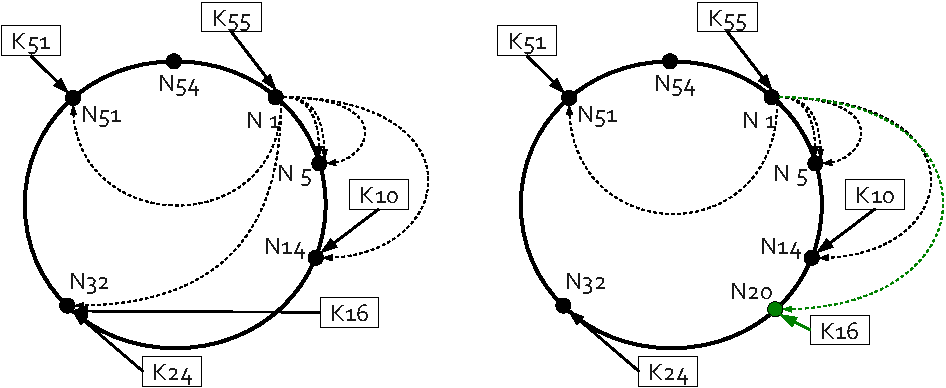
\includegraphics{grafics/chord_new_node.pdf}}
\caption{Schlüsselraum von Chord nach Ankunft von Knoten $N20$}
\label{fig:chord_new_node}
\end{figure}

\Fref[plain]{fig:chord_new_node} verdeutlicht den Neueintritt von Knoten $N20$. Die Änderungen sind in Grün dargestellt: $N1$ passt seine Fingertabelle an und $N20$ ist für $K16$ zuständig.

Der Ausfall von Knoten wird über \emph{Timeouts} ermittelt. Im Falle eines Timeouts wird die Nachricht an den besten bekannten Vorgänger des ausgefallenen Knotens weitergeleitet. Im schlimmsten Falle ist dies der Nachfolger des sendenden Knotens. Daraus wird ersichtlich, dass ein valider Nachfolger notwendig ist. Aus diesem Grund hält jeder Knoten eine Liste von möglichen Nachfolgern vor, die während \texttt{stabilize} erstellt werden. Für fehlerhafte Knoten in der Fingertabelle kann \texttt{fix\_fingers} explizit aufgerufen werden.

Knotenausfall bedeutet nicht nur einen Ausfall des Knotens, sondern bedingt, dass die dort gespeicherten Daten nicht mehr erreichbar sind.

Verlässt ein Knoten das Netz, so beeinflusst dies das System nicht. Jedoch ist es effizienter, wenn ein verlassender Knoten seinem Vorgänger und Nachfolger dies mitteilt, die Verbindungen angepasst werden und die Datensätze explizit übertragen werden.
